\textbf{Sottostringa}: serie di caratteri vicini

\textbf{Sottosequenza}: serie di caratteri non necessariamente vicini.

\section{Pattern matching di base}\label{pattern-matching-di-base}

Effettua il pattern matching esatto, cercando la sotto stringa \emph{P}
dentro la stringa \emph{T}.

\begin{breakablealgorithm}
	\caption{Ingenuo: Pattern matching ingenuo}
	\begin{algorithmic}[1]
	\Function{Ingenuo}{$ (P,T) $}
	\State $  $ \Comment{\textit{T} ha lunghezza \textit{n} e \textit{P} ha lunghezza $ m \leq n $}
	\For{$ i = 1 \: \text{to} n-m+1 $}
		\State $ j \gets 1 $
		\While{$ j \leq m \:\text{and} \:P[j] = T[i+j-1] $}
	        \State $ j \gets j + 1 $
	    \EndWhile
	    \If{$ j > m $}
	        \State Segnala l'occorrenza del pattern
	    \EndIf
	\EndFor
	\EndFunction
\end{algorithmic}
\end{breakablealgorithm}

\subsection{Utilizzo della sentinella}\label{utilizzo-della-sentinella}

La prima modifica che si può fare all'algoritmo per migliorarne
l'efficienza è quello di ridurre il test del \texttt{while}, rimuovendo
il controllo sulla lunghezza del pattern, riducendo così le operazioni
da 3 a 2.

Questo viene fatto aggiungendo una sentinella alla fine del pattern,
ovvero viene aggiunto al pattern un carattere che non compare
nell'alfabeto della stringa.

Perché questo funzioni è necessario aggiungere un carattere diverso
dalla sentinella anche alla fine di \emph{T} per permettere il match del
pattern anche quando questo è un suffisso della stringa.

\begin{breakablealgorithm}
	\caption{Ingenuo: Pattern matching ingenuo}
	\begin{algorithmic}[1]
		\Function{Ingenuo-2}{$ (P,T) $}
        \State //\textit{T} ha lunghezza \textit{n} e \textit{P} ha lunghezza $ m \leq n $
        \State $ P[m+1] \gets \$ $
        \State $ T[n+1] \gets @$
        \For{$ i = 1 \: \text{to} n-m+1 $}
	        \State $ j \gets 1 $
	        \While{$ P[j] = T[i+j-1] $}
		        \State $ j \gets j + 1 $
	        \EndWhile
	        \If{$ j > m $}
		        \State Segnala l'occorrenza del pattern
	        \EndIf
        \EndFor
        \EndFunction
\end{algorithmic}
\end{breakablealgorithm}

Nel caso non sia possibile modificare il testo si può togliere il
\texttt{+1} del ciclo \texttt{for} e sostituirlo con un \texttt{if} che
verifica l'uguaglianza dell'ultimo carattere.

D'ora in avanti assumeremo la presenza dei due caratteri sentinella.

\subsection{Riduzione del numero di confronti}\label{riduzione-del-numero-di-confronti}

Se il pattern contiene delle sottostringhe uguali, è possibile ridurre
il numero di controlli.

Ad esempio nel caso sotto riportato, l'algoritmo \textsc{Ingenuo}
effettua 20 confronti.

\begin{figure}[htbp]
\centering
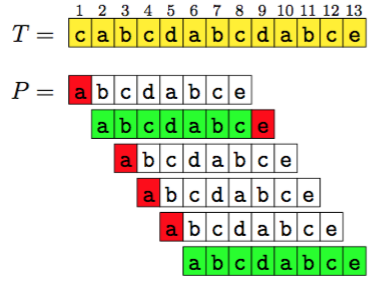
\includegraphics[width = .4\textwidth]{./notes/immagini/l11-fig1.png}
\end{figure}

Ovvero è possibile evitare il confronto tra l'inizio del pattern e il
terzo carattere del testo, perché si sa già che il terzo carattere del
testo è uguale al secondo carattere del pattern, il quale è diverso dal
primo carattere del pattern. Lo stesso ragionamento vale anche per i due
confronti successivi.

Ma si può fare di più, perché il pattern ha una sottostringa uguale al
suo prefisso, ovvero i caratteri 7-8-9 della del testo sono uguali ad
una sottostringa del pattern che coincide con il prefisso del pattern e
dal momento che questo è già questa uguaglianza è già stata verificata,
si possono ridurre ulteriormente i confronti.

\begin{figure}[htbp]
\centering
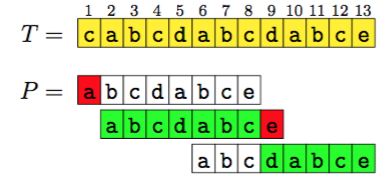
\includegraphics[width = .4\textwidth]{./notes/immagini/l11-fig2.png}
\end{figure}

Per poter applicare queste osservazioni ad un algoritmo è necessario
effettuare delle pre-elaborazioni delle stringhe.

\subsection{Pre-elaborazione fondamentale}\label{pre-elaborazione-fondamentale}

Data una stringa \emph{S} di lunghezza \emph{n}, la funzione
$\pi_i^S$ calcola la lunghezza del prefisso di \emph{S} più lungo
che occorre nella posizione \emph{i} di \emph{S}.

Quindi $\pi_i^S$ è il massimo \emph{h} tale che

$$
S[1,h] = S[i, i+h-1]
$$

Ad esempio:

\begin{figure}[htbp]
\centering
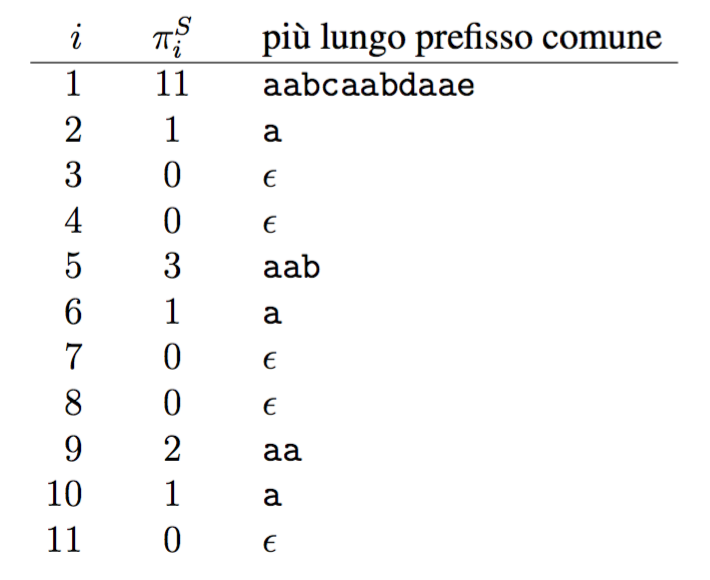
\includegraphics[width = .4\textwidth]{./notes/immagini/l11-fig3-bis.png}
\caption{$\pi_i$ per \textit{S=}\texttt{aabcaabdaae}.}
\end{figure}

Da notare che $Y = S[i, i+\pi_i -1]$ per definizione è un occorrenza in \textit{S} della stringa $S[1, \pi_i -1]$, pertanto si ha che \textit{Y} è un bordo della stringa $S[1, i +\pi_i -1]$. 
Per la relazione tra prefisso e bordo si ha quindi che $S[1, i +\pi_i -1]$ ha periodo $p = i -1$.

Si ha inoltre che la stringa $S[1, i +\pi_i -1]$ è il più lungo prefisso di \textit{S} con periodo $p= i-1$.

Questo perché se $i = 1$, si ha che il prefisso \textit{Y} coincide con \textit{S} e $p=0$, ottenendo periodo e bordo degeneri.

Se invece $ i \geq 2 $ si ha che, se $i + \pi_i -1 = n $, \textit{Y} è anche un suffisso di \textit{S}, pertanto non possono esserci altri prefissi con periodo $p = i -1$ più lunghi perché è la stringa \textit{S} è terminata.
Oppure se $i + \pi_i -1 \neq n $ vuol dire che il carattere $ S[\pi_i + 1] $ è diverso dal carattere $ S[i+\pi_i] $ per definizione di $ \pi_i $ e quindi non può esistere un prefisso $ S[1, \pi_i +1] $ con periodo $p = i -1$ perché $ S[\pi_i  + 1 + p] = S[\pi_i + i] $ che per ipotesi è diverso da $ S[\pi_i +1] $.

Le varie sottostringhe $ S[i, i + \pi_i -1 ] $ non sono necessariamente disgiunte ma possono sovrapporsi.

\subsubsection{Estremi massimi}

Fissato un $ i \geq 2 $, si ottengono varie stringhe $ S[j, j + \pi_j -1] $ con $ 2 \leq j \leq i $.

Tra tutte queste stringhe è possibile identificare la stringa che ha come valore dell' \textbf{estremo destro massimo}:

$$
r_i = \max \{ j + \pi_j -1 | \: 2 \leq j \leq i\}
$$

L'estremo sinistro associato viene indicato con 

$$
l_i = \arg\max\limits_{j} \{ j + \pi_j -1 | \: 2 \leq j \leq i\}
$$

Nel caso ci siano più sottostringhe con lo stesso estremo destro, viene scelto come estremo sinistro uno a caso tra quelli possibili.

La stringa $ S[l_i, r_i] $ risulta quindi essere la sottostringa di \textit{S} più lunga che è anche un prefisso e che inizia prima dell'indice \textit{i}.

\begin{figure}[htbp]
	\centering
	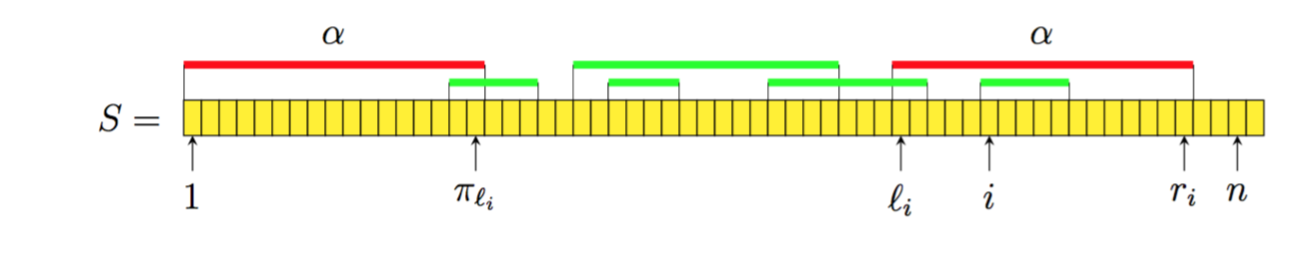
\includegraphics[width = .9\textwidth]{./notes/immagini/l11-fig4-bis.png}
	\caption{Alcune occorrenze di prefissi di \textit{S} che iniziano tra le posizioni \textit{2} e \textit{i}. L'occorrenza che termina più a destra è evidenziata in rosso.}
\end{figure}

Si ha quindi che $ S[1,r_i] $ è il più lungo prefisso di \textit{S} con periodo $ 1 \leq p < i $ e che la stringa $ S[l_i, r_i] $ è la sottostringa di \textit{S} che termina più a destra tra tutte quelle che sono uguali ad un prefisso di \textit{S}.

Ad esempio se 

$$
S = \text{\texttt{aabaabcadaabaabce}}
$$

il massimo destro con $ 2 \leq j \leq 15 $ è $ r_{15} = 10 + \pi_{10} -1 = 16$, perché $ \pi_{10} = 7$, e $ l_{15} = 10 $ che è la posizione in cui inizia la sottostringa \texttt{aabaabc}.

\subsection{Pre-elaborazione fondamentale in tempo lineare}\label{preambolazione-fondamentale-in-tempo-lineare}

Seguendo l'approccio di definizione il tempo richiesto è
$O(n^2)$, ma è possibile scendere a $O(n)$.

Supponiamo che \emph{S} termini con un carattere diverso da tutti gli
altri che compaiono nella stringa. Questo non è un problema perché si
può sempre aggiungere una sentinella.

L'algoritmo calcola $\pi_1 = n$ e poi calcola i valori $\pi_i, r_i, l_i$ per $i = 2,\ldots, n$, basandosi su un'array $ pref[1\ldots n] $ il quale conterrà i vari $ \pi_i $ e due variabili, \textit{r} e \textit{l}, le quali andranno a memorizzare gli estremi massimi tra gli indici precedente calcolati.

Come prima cosa viene effettuato il calcolo di $ \pi_2 $ confrontando da sinistra a destra i caratteri di $S[2,n]$, cosi facendo si ha che $ r = \pi_2 +1 $ e $l = 2$.

Assumendo induttivamente di aver calcolato $ \pi_j $ per ogni $ j = 2, \ldots, i-1$, si ha che $ r = r_{i-1} = \pi_{i-1} +1 $ e $ l = l_{i-1} $.

Durante il calcolo di $ \pi_i $ possono verificarsi 2 casi:

\begin{enumerate}
	\item $ i > r $: non si hanno informazioni riguardo ai caratteri che seguono \textit{i}, quindi viene effettuato il calcolo di $ \pi_i $ normalmente, andando ad effettuare i confronti da sinistra a destra tra $ S[i,n] $ e \textit{S}. Il valore di $ \pi_i $ è allora uguale alla lunghezza \textit{h} del massimo prefisso comune e $ r = i  + \pi_i +1 $ e $ l= i $.
	\item $ i \leq r$: il carattere \textit{S[i]} è contenuto nella sottostringa $ \alpha = S[l,r] $ la quale è anche prefisso di \textit{S}. Si ha quindi che il carattere \textit{S[i]} compare anche nella posizione $ i' = i - l +1 $ di \textit{S} e per lo stesso motivo la stringa $ \beta = S[i,r] $ compare anche in $ S[i', \pi_l] $.
	\begin{figure}[htbp]
		\centering
		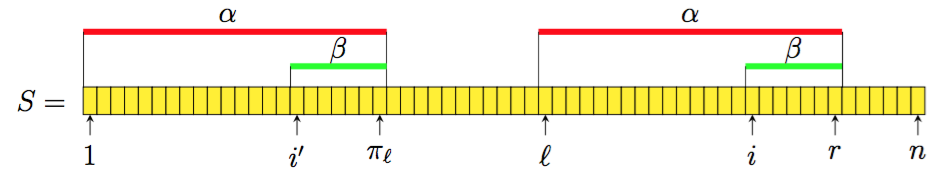
\includegraphics[width = .8\textwidth]{./notes/immagini/l11-fig3.png}
	\end{figure}
	In \textit{i'} occorrerà un prefisso $ \gamma $ di \textit{S} di lunghezza $ \pi_{i'} $, che può anche essere degenere.
	Questo prefisso occorrerà a partire dalle posizioni \textit{1} e \textit{i'} e potrà essere contenuto o contenere la sottostringa $ \beta $.
	Ne segue che \textit{S} e \textit{S[i,n]} hanno un prefisso in comune di lunghezza uguale al minimo tra $ \pi_{i'} $ e $ |\beta| = r - i +1 $.
	\begin{enumerate}
		\item $ \pi_{i'} < |\beta| $: il prefisso che inizia in \textit{i} ha la stessa lunghezza di quello che inizia in \textit{i'}, ed avendo già calcolato la lunghezza di quel prefisso si ha che $ \pi_i = \pi_{i'} $ senza effettuare alcun confronto.
		\begin{figure}[htbp]
			\centering
			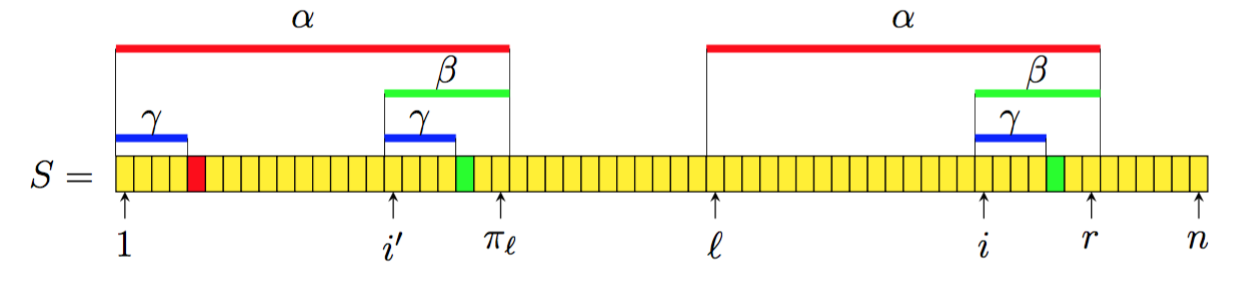
\includegraphics[width = .8\textwidth]{./notes/immagini/l11-fig5.png}
		\end{figure}
		\item $ \pi_{i'} \geq |\beta|$: l'intera sottostringa $ \beta = S[i,r] $ deve essere un prefisso di \textit{S} e quindi $\pi_i \geq |\beta| = r - i +1$. L'algoritmo calcola quindi la lunghezza \textit{h} del massimo prefisso comune tra \textit{S} e \textit{S[i,n]} a partire dai caratteri $ |\beta| + 1 $ e $ i + |\beta| $, fino a che non trova un mismatch. A questo punto vengono posti $ \pi_i =h,\: r= i + \pi_i -i \: \text{e} \: l = i $.
	\end{enumerate}
	
\end{enumerate}

\begin{breakablealgorithm}
	\caption{Prefisso: Preelaborazione del prefisso in tempo lineare}
	\begin{algorithmic}[1]
		\Function{Prefisso}{$ S $}
		    \State // S stringa di lunghezza n > 1 con sentinella alla fine
		    \State $ pref[1] \gets n $  \Comment{$ \pi_i, \pi_1 = n$}
		    \State $ h \gets 0 $
		    \While{$ S[1+h] = S[2+h] $}\Comment{Calcola $\pi_2$}
		        \State $ h = h +1 $
		    \EndWhile
		    \State $ pref[2] \gets h $
		    \State  $ l \gets 2 $
		    \State $ r \gets 2 + h - 1$
		    \For{$ i = 3 \: \text{to} \: n $}
			    \If{$ r < i $} \Comment{Caso 1}
			        \State $ h \gets 0$
		            \While{$ S[1+h] = S[i+h]$}
		                \State $ h \gets h + 1 $
		            \EndWhile
		            \State $ pref[i] \gets h$
		            \State $ l \gets i $
		            \State $ r \gets i + h -1 $
		        \Else \Comment{Caso 2}
				    \If{$pref[i-l+1] < r - i +1$} \Comment{Caso 2a}
		                \State $pref[i] \gets pref[i - l +1]$
		            \Else \Comment{Caso 2b}
		               \State $h \gets r - i +1$
		                \While{$S[1+h] = S[i +h]$}
		                    \State $ h \gets h +1 $
		                \EndWhile
		                \State $pref[i] \gets h$
		                \State $l \gets i$
		                \State $ r \gets i +h -i$
			         \EndIf
		          \EndIf
		    \EndFor
		    \State \Return $ pref $
		   \EndFunction
	\end{algorithmic}
\end{breakablealgorithm}

La correttezza dell'algoritmo deriva da quanto detto prima

\paragraph{Complessità}\label{complessituxe0}

Se non viene presa in considerazione la complessità dei cicli
\texttt{while} si ha che la complessità è data da \emph{O(n)}.

I cicli \texttt{while} terminano quando viene trovato un mismatch e al
massimo vengono trovati \emph{n-1} mismatch (1 dal \texttt{while}
esterno, $n-2$ dai \texttt{while} dentro il ciclo \texttt{for}).

Ad ogni confronto con successo, il carattere destro ($S[i+h]$)
viene spostato a destra di 1 e, una volta terminato il \texttt{while}, questo viene posto a $r = i + h - 1$, ovvero risulta essere il carattere alla posizione $S[r+1]$.

All'iterazione successiva il ciclo \texttt{while} inizia con carattere destro $S[i]$ se $i > r$\footnote{Viene quindi sposto a destra perché $ i \geq r+1 $} altrimenti inizia con $S[i + h]$ con $h = r - i + 1$. In entrambi i casi il carattere destro non si sposta mai a sinistra durante l'esecuzione dell'algoritmo. 
Pertanto vengono eseguiti al più $n-1$ confronti con successo. +
Si ottiene quindi una complessità per i \texttt{while} di $O(2n-2)$.

La complessità totale dell'algoritmo è data da $O(n) +\textit{ Complessità while }= O(n) + O(2n-2) = O(n)$.

\subsubsection{Matching esatto in tempo lineare}\label{matching-esatto-in-tempo-lineare}

Per effettuare il pattern matching in tempo $O(m+n)$ del pattern \emph{P} in \emph{T} è possibile utilizzare una versione leggermente modifica della funzione prefisso sulla stringa \emph{S = P\$T}, dove \$ è un simbolo che non è presente nelle due stringhe.

Questo viene fatto calcolando $ \pi_i^S $ per $ i = 2, \ldots n + m +1 $.
Siccome \$ non compare in nessuna delle due stringhe, si ha che $ \pi_i \leq m \: \forall \: i $ perché per ipotesi la sottostringa \textit{P\$} non può comparire all'interno di \textit{T}.
Inoltre, $ \forall \: i \geq m +1 : \pi_i = m $ si ha che $i - m - 1$ identifica l'inizio di un'occorrenza di \textit{P} in \textit{T}, perché $ \pi_i = m $ indica la presenza di prefisso di lunghezza \textit{m} a partire dalla posizione \textit{i}, ma la sottostringa prefissa di lunghezza \textit{m} coincide per costruzione con \textit{P}, quindi \textit{i} indica l'inizio di un'occorrenza del pattern \textit{P} nella stringa \textit{P\$T}.

Dal momento che il prefisso viene calcolato in tempo lineare rispetto la lunghezza della stringa, si ottiene una funzione di pattern matching con complessità lineare.

Altre caratteristiche di questo algoritmo sono:
\begin{itemize}
	\item il \textbf{consumo lineare di memoria} rispetto la lunghezza del pattern $ O(m) $, perché è possibile evitare di tenere in memoria tutti $ \pi_i $ con $ i >m $ perché tutti i valori \textit{i'} del caso 2 faranno sempre riferimento ai $ \pi_i \: \text{con}\: i \leq m $
	\item che non è necessario conoscere tutto l'alfabeto, basta avere la possibilità di confrontare i caratteri.
\end{itemize}

\subsubsection{Esercizio - Identificare una rotazione}

Date due stringhe \textit{X} ed \textit{Y} di uguale lunghezza \textit{n}, determinare in tempo lineare \textit{O(n)}, se \textit{Y} è una rotazione circolare di \textit{X}.
Ovvero se è possibile identificare due stringhe $ \alpha $ e $ \beta $ tali che $ X = \alpha\beta $ e $ Y = \beta\alpha $.

\paragraph{Soluzione}

Si concatenano le stringhe in modo da formare $ S = Y\$XX $, se eseguendo la preelaborazione trovo un prefisso di lunghezza \textit{n} a partire dal $n+1$ vuol dire che \textit{Y} compare tra le due \textit{X} e quindi le due stringhe sono la rotazione di una stessa stringa.

\subsubsection{Esercizio - Massima sottostringa comune}

Date due stringhe \textit{X} e \textit{Y} di lunghezza \textit{m} e \textit{n} calcolare, in tempo lineare, il più lungo suffisso di \textit{X} che è anche prefisso di \textit{Y}. 
Ovvero la sottostringa $ \gamma $ di lunghezza massima tale che $ X = \alpha\gamma \: \text{e} \: Y = \gamma\alpha$.

\paragraph{Soluzione}

L'idea è quella di concatenare due stringhe in modo da formare $ S= Y\$X $, dove \$ è un carattere che non compare in nessuna delle due stringhe, per poi effettuare la preelaborazione.

Se $ \pi_2^S = 0$ non c'è nessuna sottostringa uguale al prefisso di \textit{Y}, quindi $ \gamma = \epsilon $, altrimenti se  $ 0 < \pi_2^S = k \leq m$ si ha che c'è un'occorrenza all'interno di \textit{S} del prefisso di \textit{Y} lunga \textit{k}, ma non si ha alcuna garanzia che questa sia un suffisso per \textit{X}.

Se  $ \pi_{n+m+1-k}^S = k$ si ha che a partire dal carattere $ n+m+1-k $ c'è un match di una sottostringa di lunghezza \textit{k} che per costruzione è anche suffisso di \textit{X}, pertanto $ \gamma = Y[1,k] $, altrimenti la sottostringa precedentemente identifica si trova o all'interno di \textit{Y} o all'interno di \textit{X}, pertanto $ \gamma = \epsilon $.

\todo[inline]{Quasi corretto, bisogna andare a vedere i $ \pi_j $ per trovare il suffisso più lungo che è anche prefisso.}


